\documentclass[border=3pt]{standalone}
\usepackage{tikz}
\usepackage{amsmath}
\usetikzlibrary{arrows.meta,calc,positioning}

\definecolor{brandred}{RGB}{204,0,0}
\definecolor{brandblue}{RGB}{0,0,170}

\tikzset{
  flowarrow/.style={-{Stealth[length=3mm]},line width=0.8pt},
  axisarrow/.style={-Stealth,line width=0.5pt},
  bell/.style={line width=0.8pt},
  caption/.style={font=\footnotesize,align=center},
  dot/.style={circle,fill,inner sep=1.2pt}
}

% 一个简化的“分布小面板”命令:在 x=<#1> 处绘制曲线和说明文字
\newcommand{\PreferencePanel}[3]{%
  \begin{scope}[shift={(#1,0)},scale=#3]
    % 基线(示意坐标轴,向右箭头)
    \draw[axisarrow] (-1.2,0) -- (1.6,0);
    % 钟形曲线(示意)
    \draw[bell]
      plot[domain=-0.95:0.95,samples=140]
        (\x,{1.05*exp(-(\x*\x)/0.32)});
    % 下方说明
    \node[caption] at (0,-0.65) {#2};
  \end{scope}%
}

\begin{document}
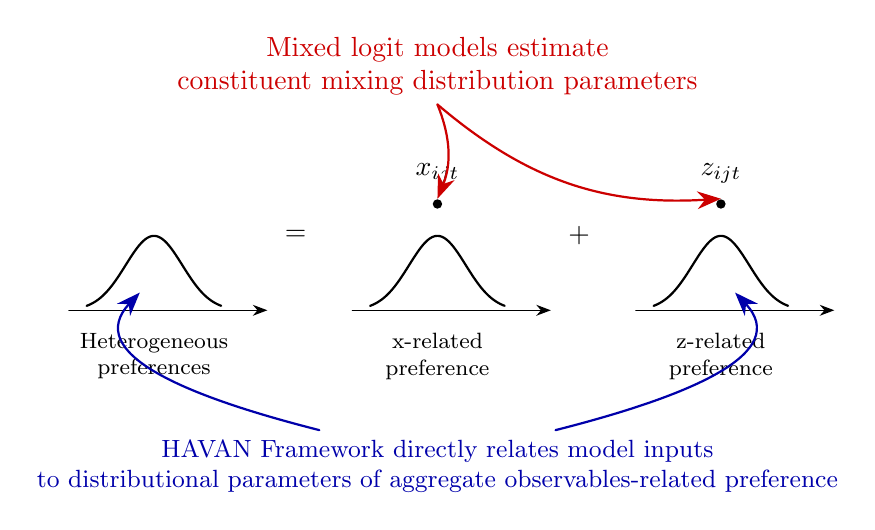
\begin{tikzpicture}[x=0.9cm,y=0.9cm,line cap=round,line join=round]
  % 三个分布面板
  \PreferencePanel{-4}{Heterogeneous\\preferences}{1.0}
  \PreferencePanel{0}{x-related\\preference}{1.0}
  \PreferencePanel{4}{z-related\\preference}{1.0}

  % 等号与加号(高度略高于曲线峰)
  \node at (-2,1.05) {$=$};
  \node at ( 2,1.05) {$+$};

  % 黑点与变量标签(位于中、右面板上方)
  \node[dot] (xpt) at (0,1.50) {};
  \node[above=2pt of xpt] {$x_{ijt}$};
  \node[dot] (zpt) at (4,1.50) {};
  \node[above=2pt of zpt] {$z_{ijt}$};

  % 顶部红色标题
  \node[text=brandred,align=center] (toptext) at (0,3.45)
    {Mixed logit models estimate\\
     constituent mixing distribution parameters};

  % 从顶部文字到两个黑点的红色弧线箭头
  \draw[flowarrow,draw=brandred]
    (toptext.south) to[bend left=22] (xpt.north);
  \draw[flowarrow,draw=brandred]
    (toptext.south) to[bend right=22] (zpt.north);

  % 底部蓝色说明
  \node[text=brandblue,align=center,font=\small] (bottomtext) at (0,-2.20)
    {HAVAN Framework directly relates model inputs\\
     to distributional parameters of aggregate observables-related preference};

  % 从底部说明到左右面板的长弧形蓝色箭头(U 形)
  \coordinate (L) at (-4.2,0.25);
  \coordinate (R) at ( 4.2,0.25);
  \draw[flowarrow,draw=brandblue]
    ([xshift=-1.5cm]bottomtext.north) .. controls (-3.6,-1.2) and (-5.0,-0.6) .. (L);
  \draw[flowarrow,draw=brandblue]
    ([xshift= 1.5cm]bottomtext.north) .. controls ( 3.6,-1.2) and ( 5.0,-0.6) .. (R);
\end{tikzpicture}
\end{document}